\documentclass[11pt]{article}

\usepackage{custom}

\title{605.744: Information Retrieval \\ Programming Assignment \#5: Near Duplicate Detection}
\author{Sabbir Ahmed}
\date{\today}

\begin{document}
\maketitle
\tableofcontents
\clearpage
\newpage

\section{Introduction}
This paper describes the classification of the Systematic Review dataset through exploratory analysis, grid searching for optimal estimators and their hyperparameters, and determining the best features.

% \section{Technical Background}
% All of the source code is in Python 3.10. The program is split into several modules and follows an object oriented structure.

% % .
% % ├── ir/
% % │   ├── __init__.py
% % │   ├── files.py
% % │   ├── metrics.py
% % │   ├── model.py
% % │   └── normalize.py
% % ├── models/
% % ├── outputs/
% % └── run.py

% \begin{figure}[!ht]
%     \centering
%     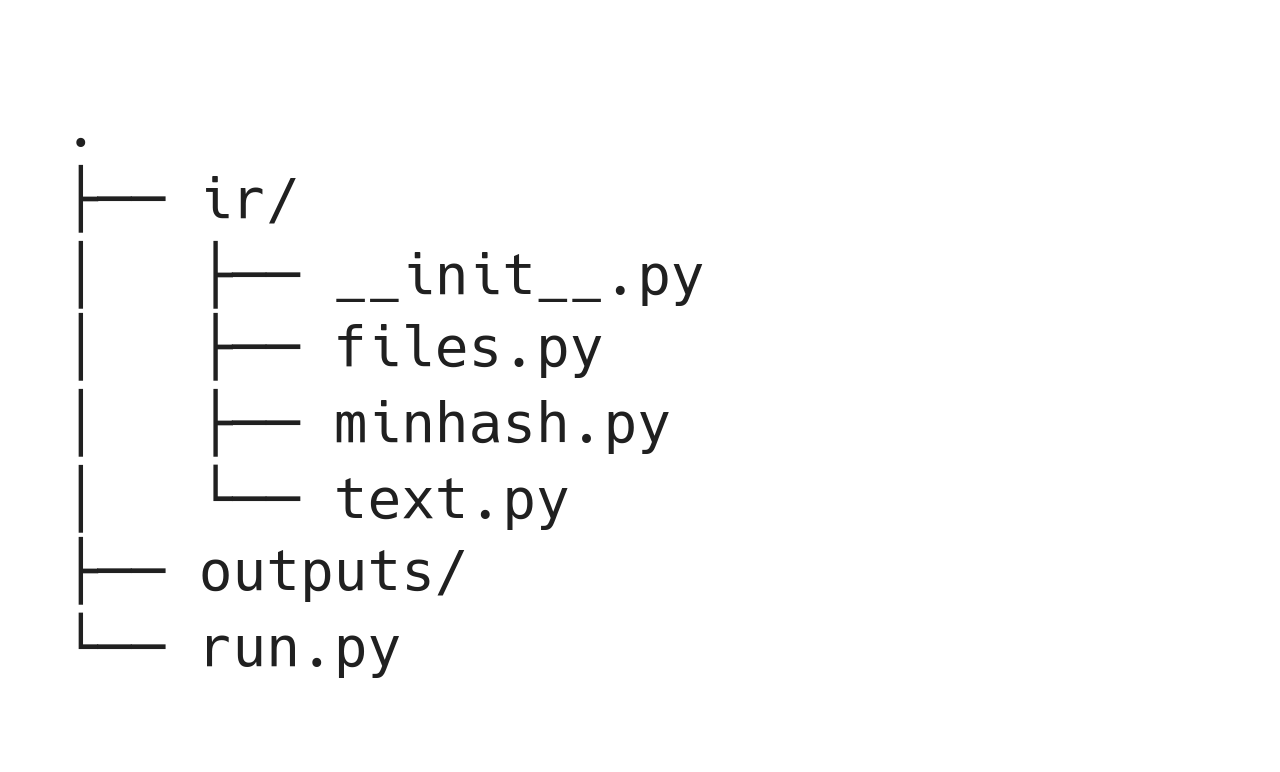
\includegraphics[trim={0 0 15cm 3cm},clip,scale=0.3]{statics/dirtree.png}
%     \caption{Directory Hierarchy of Assignment 4}
% \end{figure}

% The source code for all of the files are attached in Appendix \ref{appendix:src}.

% The total number of non-empty lines of code for the program totals to under 460.

% \begin{figure}[!ht]
%     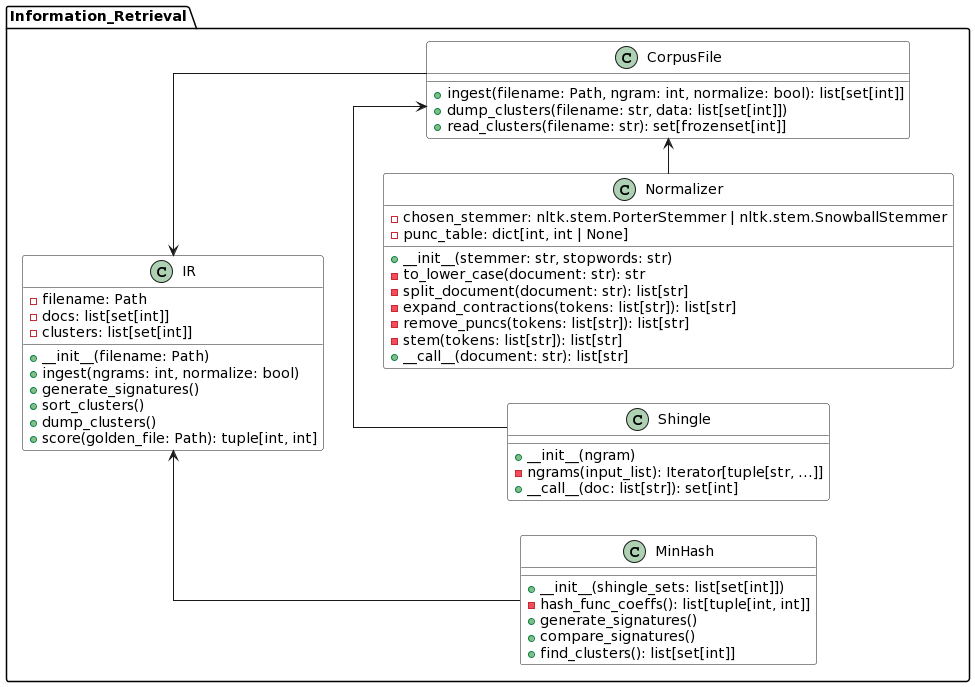
\includegraphics[scale=0.35]{statics/uml.png}
%     \centering
%     \caption{UML of Information Retrieval}
% \end{figure}

% \subsection{Classes}
% Some classes from Assignment 3 were used in this project:
% \begin{itemize}
%     \item the driver script \texttt{run.py} was modified with the relevant flags
%     \item the methdods in \texttt{files.IO} were simplified to handle only plain text and joblib binaries
%     \item the \texttt{files.CorpusFile} class was modified to process TSV files and transform the content into a list of mapped values
%     \item the \texttt{normalize.Normalizer} class was used to compare text tokenization methods
%     \item the \texttt{lexer} classes were replaced by the \texttt{CountVectorizer} class provided by \texttt{scikit-learn}
% \end{itemize}

% \subsection{External Libraries}
% The following external libraries were used to implement portions of the assignment:
% \begin{itemize}
%     \item Natural Language Toolkit (NLTK) \cite{bird2009natural}
%     \item scikit-learn (sklearn) \cite{scikit-learn}
%     \item XGBoost \cite{Chen_2016}
% \end{itemize}

% \section{Exploratory Analysis}
% The dataset is a collection of tab separated value (TSV) files with 10 features. The training portion is used to train the models, the development portion is used to score the performances of the models, and the test portion is used for its target features to be predicted by the models. 

% \begin{simptable}
%     {Description of the features of the Systematic Review dataset}
%     {features}
%     {| l | l |}
%     \textbf{Feature} & \textbf{Description}
%     \\ \hline
%     Assessment & -1, 0, or 1; zero indicates unknown; 1=accept, -1=reject
%     \\ \hline
%     DocID & Unique ID. Usually PubMed ID, or hashed ID
%     \\ \hline
%     Title & Article title
%     \\ \hline
%     Authors & List of authors
%     \\ \hline
%     Journal & Journal title
%     \\ \hline
%     ISSN & Numeric code for journal
%     \\ \hline
%     Year & Publication year
%     \\ \hline
%     Language & Trigram for language code (e.g., "eng")
%     \\ \hline
%     Abstract & Several sentence abstract from article
%     \\ \hline
%     Keywords & List of keywords
%     \\ \hline
% \end{simptable}

% The \textit{Assessment} feature in the training and development datasets is the target binary value, and will be predicted for the testing dataset. The feature is heavily imbalanced, with Table \ref{table:dist_train} showing the distribution in the training dataset:

\begin{simptable}
  {Distribution of \textit{Assessment} in the training dataset}
  {dist_train}
  {| c | c | c |}
  \textbf{N-Gram} & \textbf{Normalized} & \textbf{Score}
  \\ \hline
  \textbf{1} & True & (2, 1)
  \\ \hline
  \textbf{1} & False & (2, 2)
  \\ \hline
  \textbf{2} & True & (1, 2)
  \\ \hline
  \textbf{2} & False & (3, 2)
  \\ \hline
  \textbf{3} & True & (2, 4)
  \\ \hline
  \textbf{3} & False & (2, 4)
  \\ \hline
  \textbf{4} & True & (3, 6)
  \\ \hline
  \textbf{4} & False & (3, 6)
  \\ \hline
  \textbf{5} & True & (3, 6)
  \\ \hline
  \textbf{5} & False & (4, 9)
  \\ \hline
  \textbf{6} & True & (10, 12)
  \\ \hline
  \textbf{6} & False & (10, 12)
  \\ \hline
\end{simptable}

% The following features are considered text features, where they are represented as single strings:
% \begin{itemize}
%     \item DocID
%     \item Title
%     \item Year
%     \item Language
%     \item Abstract
% \end{itemize}

% The following features are considered list of text features, where they are represented as string lists:
% \begin{itemize}
%     \item Authors
%     \item Journal
%     \item ISSN
%     \item Keywords
% \end{itemize}

% \section{Classification Algorithms}
% For classification, machine learning algorithms implemented by \texttt{scikit-learn} were used.

% For text tokenizing and normalizing, the \texttt{CountVectorizer} and \texttt{TfidfTransformer} classes by \texttt{scikit-learn} were used. \texttt{CountVectorizer} ingested text values and created bags-of-words. This data structure was further transformed using \texttt{TfidfTransformer} to assign TF-IDF values to the terms in the vocabulary.

% \subsection{Scoring}
% To compare performances of the models, the following metrics were emphasize:
% \begin{itemize}
% \setlength\itemsep{1em}
%     \item Precision (P): $ \dfrac{TP}{TP + FP} $
%     \item Recall (R): $ \dfrac{TP}{TP + FN} $
%     \item F1-score: $ 2 \cdot \dfrac{P \cdot R}{P+R} $
% \end{itemize}

% These scores are computed in \texttt{metrics.Metrics}.

% \section{Experiments}

% \subsection{Baseline}
% For the initial phase, only the \textit{Title} feature was used as the feature. As a text feature, each of the values were tokenized, vectorized, and their TF-IDF values were used to predict the corresponding target value. The previously implemented \texttt{normalize.Normalizer} class was used as the tokenizer to \texttt{CountVectorizer}.

% The text vectorizers from \texttt{scikit-learn} were used with their default parameters. For classification, the linear support vector machine (SVM) with stochastic gradient descent (SGD), \\
% \texttt{SGDClassifier(loss="hinge")} was used.

% To account for the skewed data, an additional parameter $class\_weight=\{1:30\}$ was used.

% Table \ref{table:base_score} lists the model's scores:

% \begin{simptable}
%     {Scores using only \textit{Title} as the feature}
%     {base_score}
%     {| c | c |}
%     \textbf{Metric} & \textbf{Score}
%     \\ \hline
%     Precision & 0.195 
%     \\ \hline
%     Recall & 0.640
%     \\ \hline
%     F1-Score & 0.299
%     \\ \hline

% \end{simptable}

% \subsection{Experiment \#1: More Features}
% To improve the scores of the model, the features \textit{Abstract} and \textit{Keywords} were added. The vocabulary from the 3 features were merged and tokenized through the vectorizers. 

% Table \ref{table:gs0_score} lists the model's scores:

% \begin{simptable}
%     {Scores using \textit{Title}, \textit{Abstract} and \textit{Keywords} as the features}
%     {gs0_score}
%     {| c | c |}
%     \textbf{Metric} & \textbf{Score}
%     \\ \hline
%     Precision & 0.330 
%     \\ \hline
%     Recall & 0.747
%     \\ \hline
%     F1-Score & 0.458
%     \\ \hline
% \end{simptable}

% \subsection{Experiment \#2: Hyperparameter Optimization and Feature Selection}
% In addition to the features, the grid searching algorithm by scikit-learn, \texttt{GridSearchCV}, was used to find the best-performing hyperparameters. The following parameters were used:
% \begin{enumerate}
%     \item Tokenizer for \texttt{CountVectorizer}:
%     \begin{enumerate}
%         \item With one of the following stemmers:
%         \begin{enumerate}
%             \item No stemming
%             \item Snowball stemmer
%             \item Porter stemmer
%         \end{enumerate}
%         \item Combined with the following stop words list options:
%         \begin{enumerate}
%             \item No stopwords removed
%             \item Custom stop words list generated from previous assignments
%             \item English stop words provided by scikit-learn
%         \end{enumerate}
%     \end{enumerate}
%     \item Class weight for \texttt{SGDClassifier}: $\{\{1: i\}, 3 \le i \le 30\}$
% \end{enumerate}
% In total, 196 combinations were exhaustively searched to find the optimal F1-score.

% Along with the hyperparameter search, various combinations of features were tested as well. Features such as \textit{Authors} and \textit{Year} do not appear to contribute to the model's performance, and \textit{Journal} appears to degrade the performance. The optimal features were determined to be: \{\textit{Title}, \textit{Abstract}, \textit{Keywords}, \textit{Language}\}.

% Figure \ref{fig:cv} lists the scores yielded by the various combinations of class weight ratios, tokenization methods, and stop words lists. The scores are the mean F1-scores of the 5-fold cross validation segments.

% \begin{figure}[!ht]
%     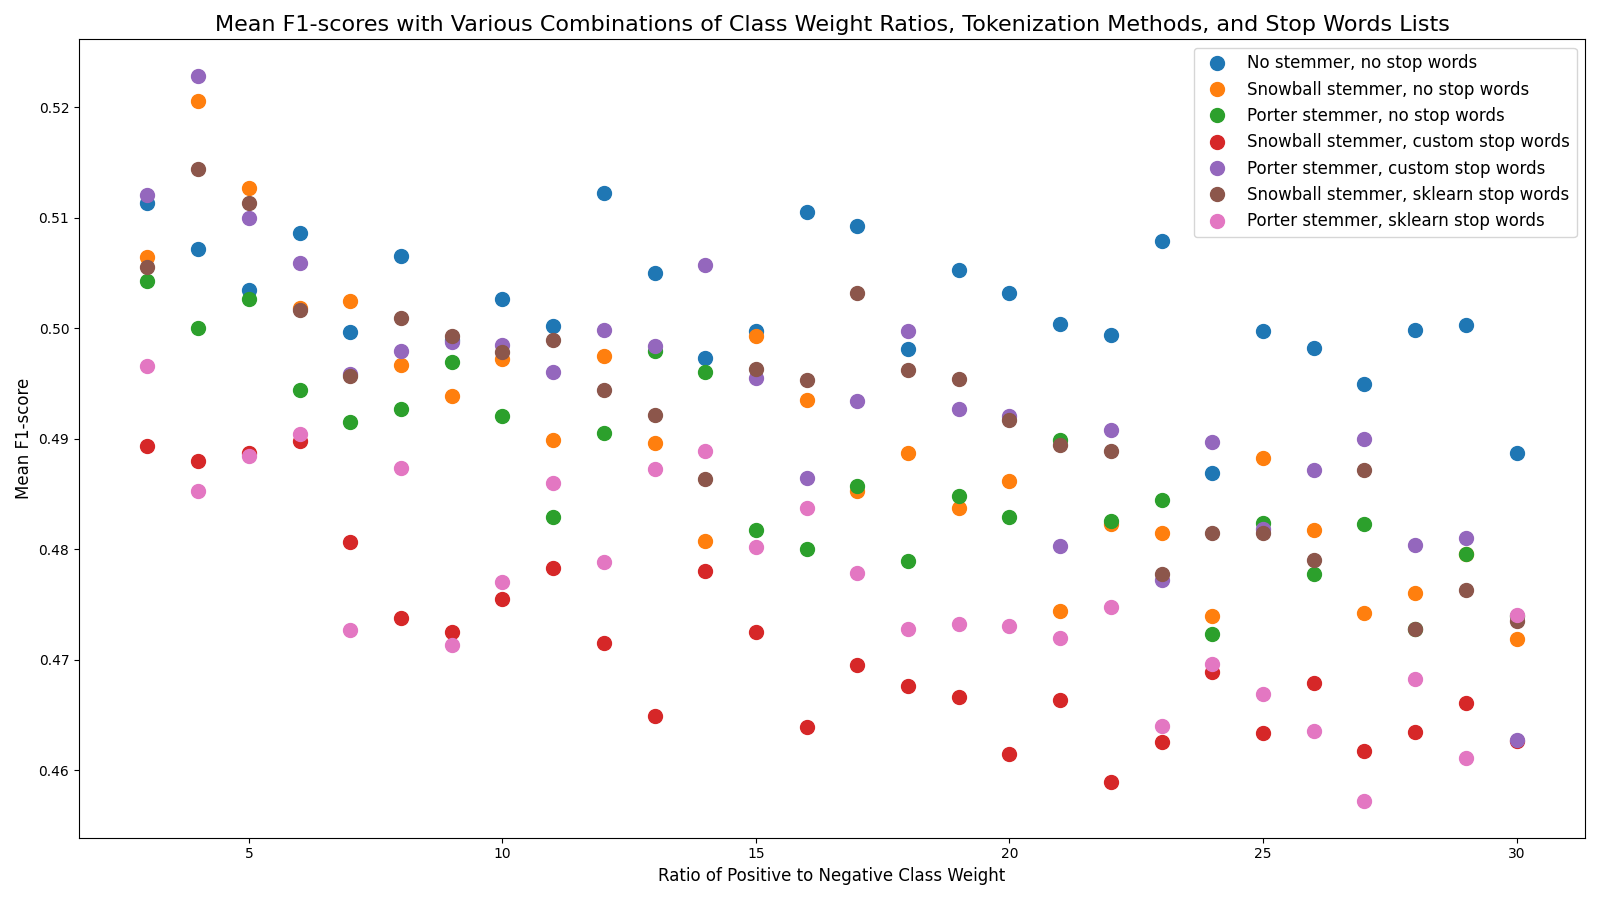
\includegraphics[scale=0.46]{statics/cv.png}
%     \centering
%     \caption{Mean F1-scores with Various Combinations of Class Weight Ratios, Tokenization Methods, and Stop Words Lists}
%     \label{fig:cv}
% \end{figure}

% Table \ref{table:gs1_param} lists the parameters with the best scores.
% \begin{simptable}
%     {Optimal parameters determined via grid search}
%     {gs1_param}
%     {| l | c |}
%     \textbf{Parameter} & \textbf{Value}
%     \\ \hline
%     Stemmer for \texttt{CountVectorizer} & Snowball
%     \\ \hline
%     Stop words list & None
%     \\ \hline
%     Class weight ratio for \texttt{SGDClassifier} & \{1: 4\}
%     \\ \hline
% \end{simptable}

% The tokenizer, when not using any stemming or stop words lists perform the best consistently. Some models, such as the tokenizer with either of the stemmers and no stop words lists, appear to perform well with low weight classes, but degrade over increasing weights.

% Table \ref{table:gs1_score} shows the optimal model's scores.
% \begin{simptable}
%     {Scores using \textit{Title}, \textit{Abstract}, \textit{Keywords} and \textit{Language} as the features}
%     {gs1_score}
%     {| c | c |}
%     \textbf{Metric} & \textbf{Score}
%     \\ \hline
%     Precision & 0.503 
%     \\ \hline
%     Recall & 0.587
%     \\ \hline
%     F1-Score & 0.542
%     \\ \hline
% \end{simptable}

% \subsubsection{Analysis}
% The exhaustive grid search yielded an optimal model with an F1-score of 0.542. When hyperparameter tuning, all of the 3 metrics were initially considered (precision, recall, and F1-score) but it ranked models with inconsistent performances on the development dataset, i.e models with recall of >0.8 yielded precision of <0.2. The models had to be narrowed down to just the F1-scores.

% \subsection{Experiment \#3: eXtreme Gradient Boosting}
% An additional experiment was performed, where the same features were trained on an XGBoost (eXtreme Gradient Boosting) estimator \cite{Chen_2016}. A similar approach to hyperparameter tuning and feature selection with the SVM model was taken with this estimator, although not as thoroughly due to memory and time constraints.

% \begin{simptable}
%     {Optimal parameters determined via grid search}
%     {gs2_param}
%     {| c | c |}
%     \textbf{Metric} & \textbf{Score}
%     \\ \hline
%     objective & binary:logistic
%     \\ \hline
%     scale\_pos\_weight & 3
%     \\ \hline
%     learning\_rate & 0.2
%     \\ \hline
%     n\_estimators & 100
%     \\ \hline
%     max\_depth & 3
%     \\ \hline
%     min\_child\_weight & 10
%     \\ \hline
%     max\_delta\_step & 3
%     \\ \hline
%     subsample & 0.8
%     \\ \hline
% \end{simptable}

% Table \ref{table:gs2_score} shows the optimal model's scores.

% \begin{simptable}
%     {Scores using \textit{Title}, \textit{Abstract}, \textit{Keywords} and \textit{Language} as the features}
%     {gs2_score}
%     {| c | c |}
%     \textbf{Metric} & \textbf{Score}
%     \\ \hline
%     Precision & 0.631 
%     \\ \hline
%     Recall & 0.433
%     \\ \hline
%     F1-Score & 0.514
%     \\ \hline
% \end{simptable}

% \subsubsection{Analysis}
% The scores yielded did not appear to be significantly different from the SVM model, although recall can be prioritized by adjusting properties of the tree structures such as \texttt{max\_depth} and \texttt{min\_child\_weight}.

% \section{Conclusion}
% The SVM model with the optimal parameters appeared to perform the best. Ultimately, this model was used to predict the target values of the test portion of the dataset. The predictions were saved to the attached file, \texttt{sahmed80.txt}.

% \addcontentsline{toc}{section}{References}
% \bibliographystyle{ieeetr}
% \bibliography{refs}

% \appendix
% \addcontentsline{toc}{section}{Appendix}%

% \section{Source Code} \label{appendix:src}

% \inputpython{../ir/\_\_init\_\_.py}{ir/\_\_init\_\_.py}
% \inputpython{../ir/files.py}{ir/files.py}
% \inputpython{../ir/metrics.py}{ir/metrics.py}
% \inputpython{../ir/normalize.py}{ir/normalize.py}
% \inputpython{../ir/model.py}{ir/model.py}

% \inputpython{../run.py}{run.py}

\end{document}
